\documentclass[twoside,10pt]{article}
\usepackage{/Users/bradenhoagland/latex/styles/toggles}
%\toggletrue{sectionbreaks}
%\toggletrue{sectionheaders}
\newcommand{\docTitle}{Math 323 - HW 6}
\usepackage{/Users/bradenhoagland/latex/styles/common}
\importStyles{modern}{rainbow}{boxy}

%\renewcommand{\theenumi}{\alph{enumi}}

\begin{document}
%\tableofcontents

% ------------------------------
% 3.5
% ------------------------------
\begin{exer}[3.5]
Construct a square with side length 1.
\end{exer}

\begin{figure}[H]
	\centering
	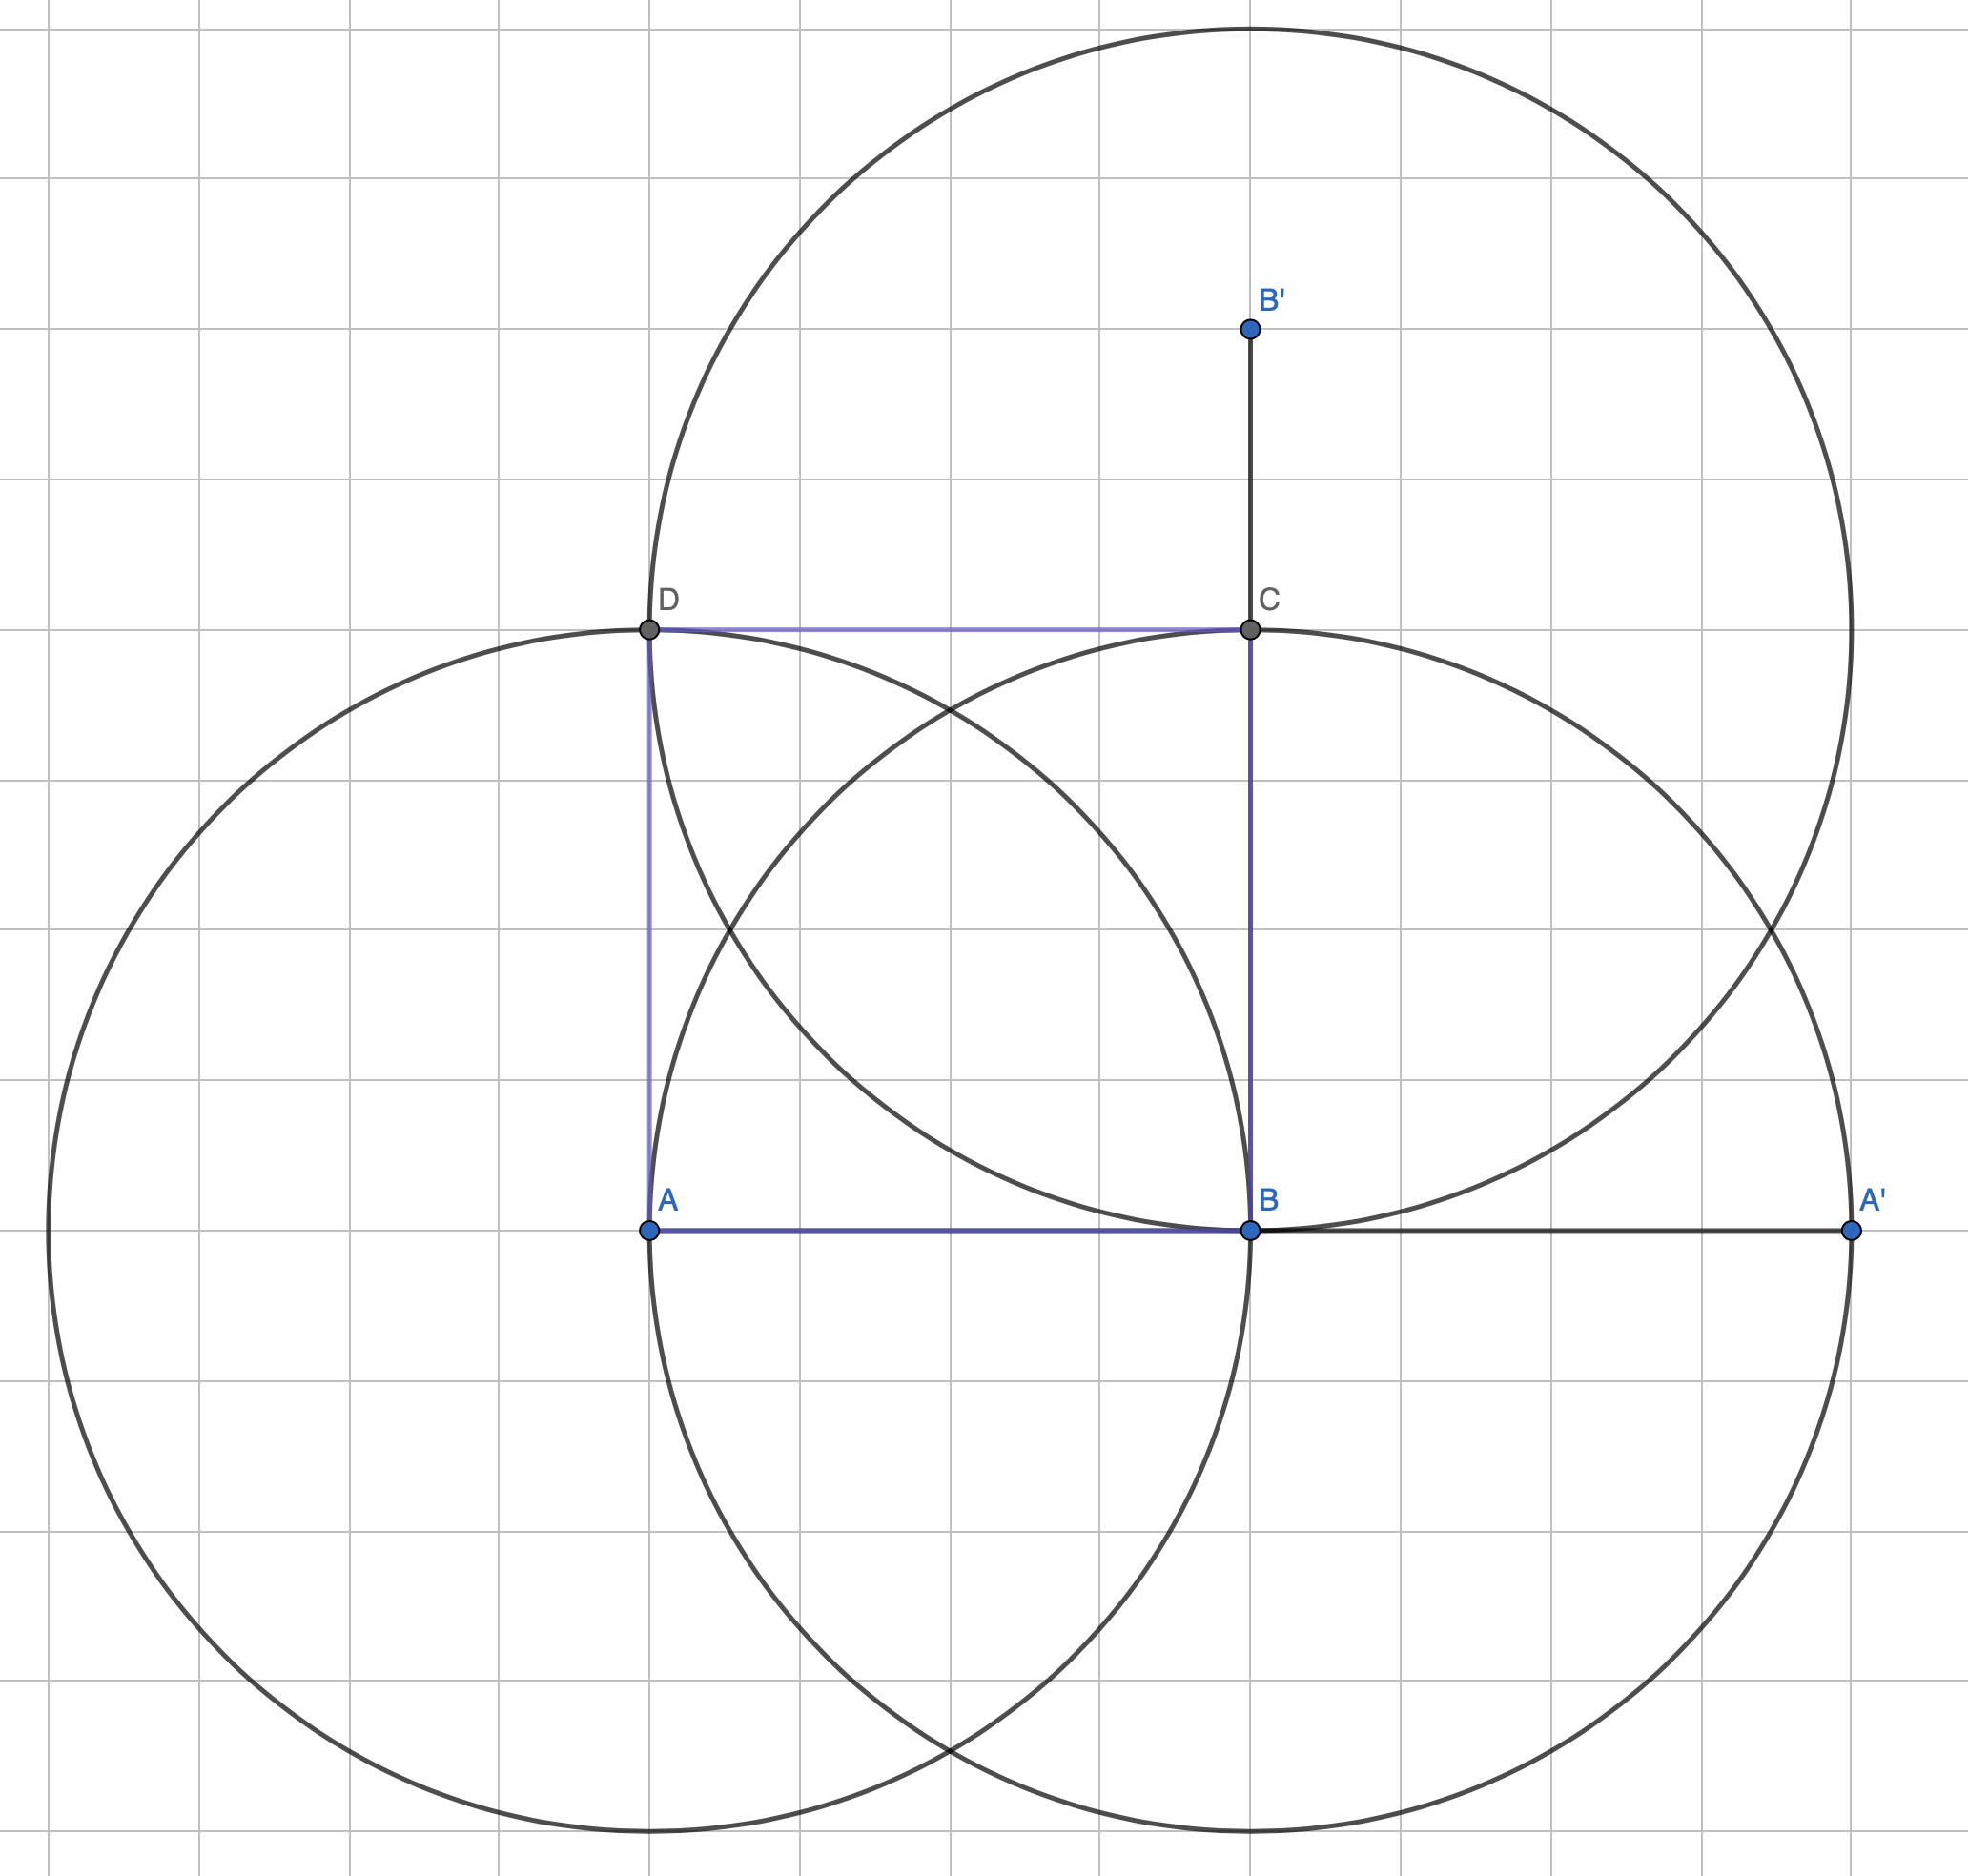
\includegraphics[scale=0.2]{fig/5}
	%\caption{}
\end{figure}

Suppose $|AB|=1$, then extend this line, then construct the point $A'$ that is on the intersection of $\mathcal{C}_B(|AB|)$. By Lemma 3.7, we can construct the perpendicular bisector to this line, which must necessarily pass through $B$. Let $C$ be one of the two points on the perpendicular bisector of $AA'$ that intersects $\mathcal{C}_B(|AB|)$. Now let $ D$ be the point of intersection (other than $B$) of $\mathcal{C}_C(|BC|)$ and $\mathcal{C}_A(|AB|)$. The quadrilateral $ABCD$ is then a square with side length $|AB|=1$.

\newpage

% ------------------------------
% 3.16
% ------------------------------
\begin{exer}[3.16]
Construct a regular octagon.
\end{exer}

By the previous exercise, we know we can construct a square, so do that and label its edges $A,B,C,D$. Construct the diagonals and label their intersection $O$.

\begin{figure}[H]
	\centering
	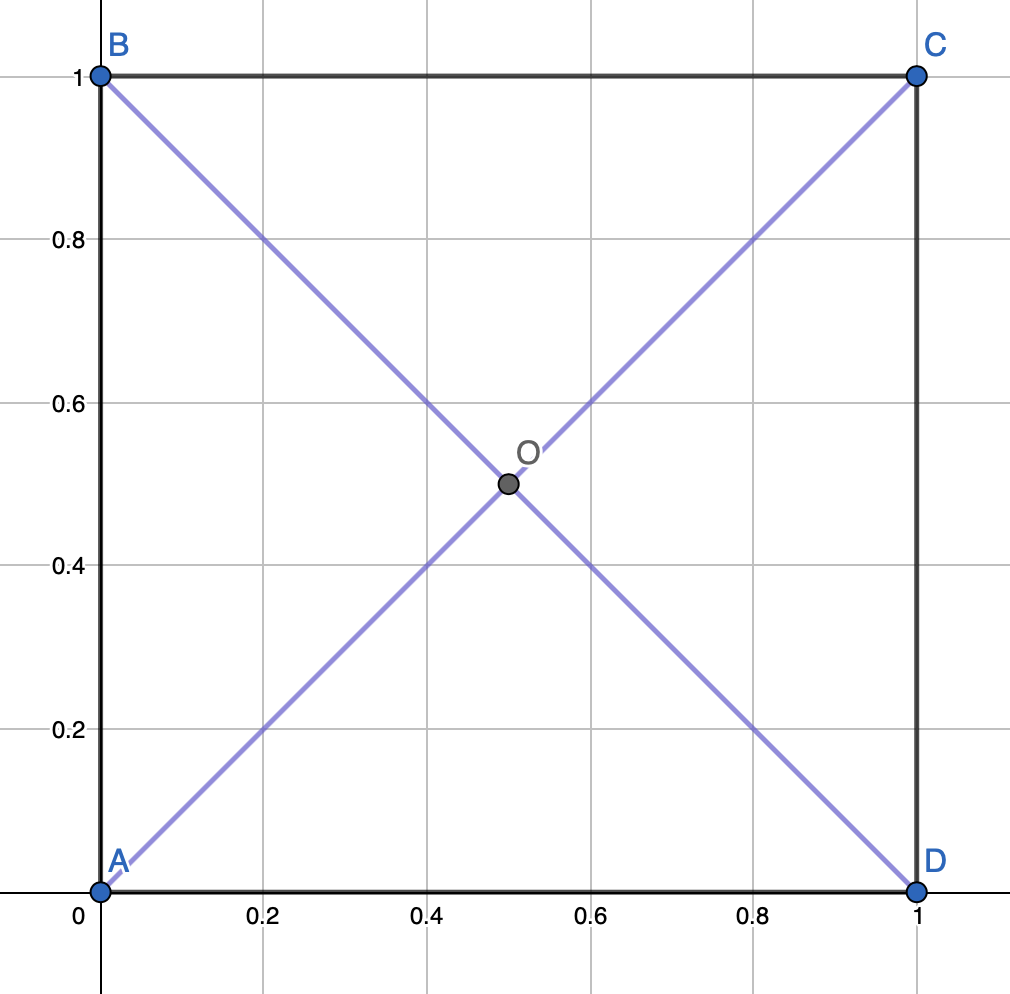
\includegraphics[scale=0.3]{fig/16a}
	%\caption{}
\end{figure}

Now construct the four circles $\mathcal{C}_{A}(|AO|), \mathcal{C}_{B}(|BO|), \mathcal{C}_{C}(|CO|),$ and $\mathcal{C}_{D}(|DO|)$. The 8 intersection points of these circles with the square form a regular hexagon, pictured in red below.

\begin{figure}[H]
	\centering
	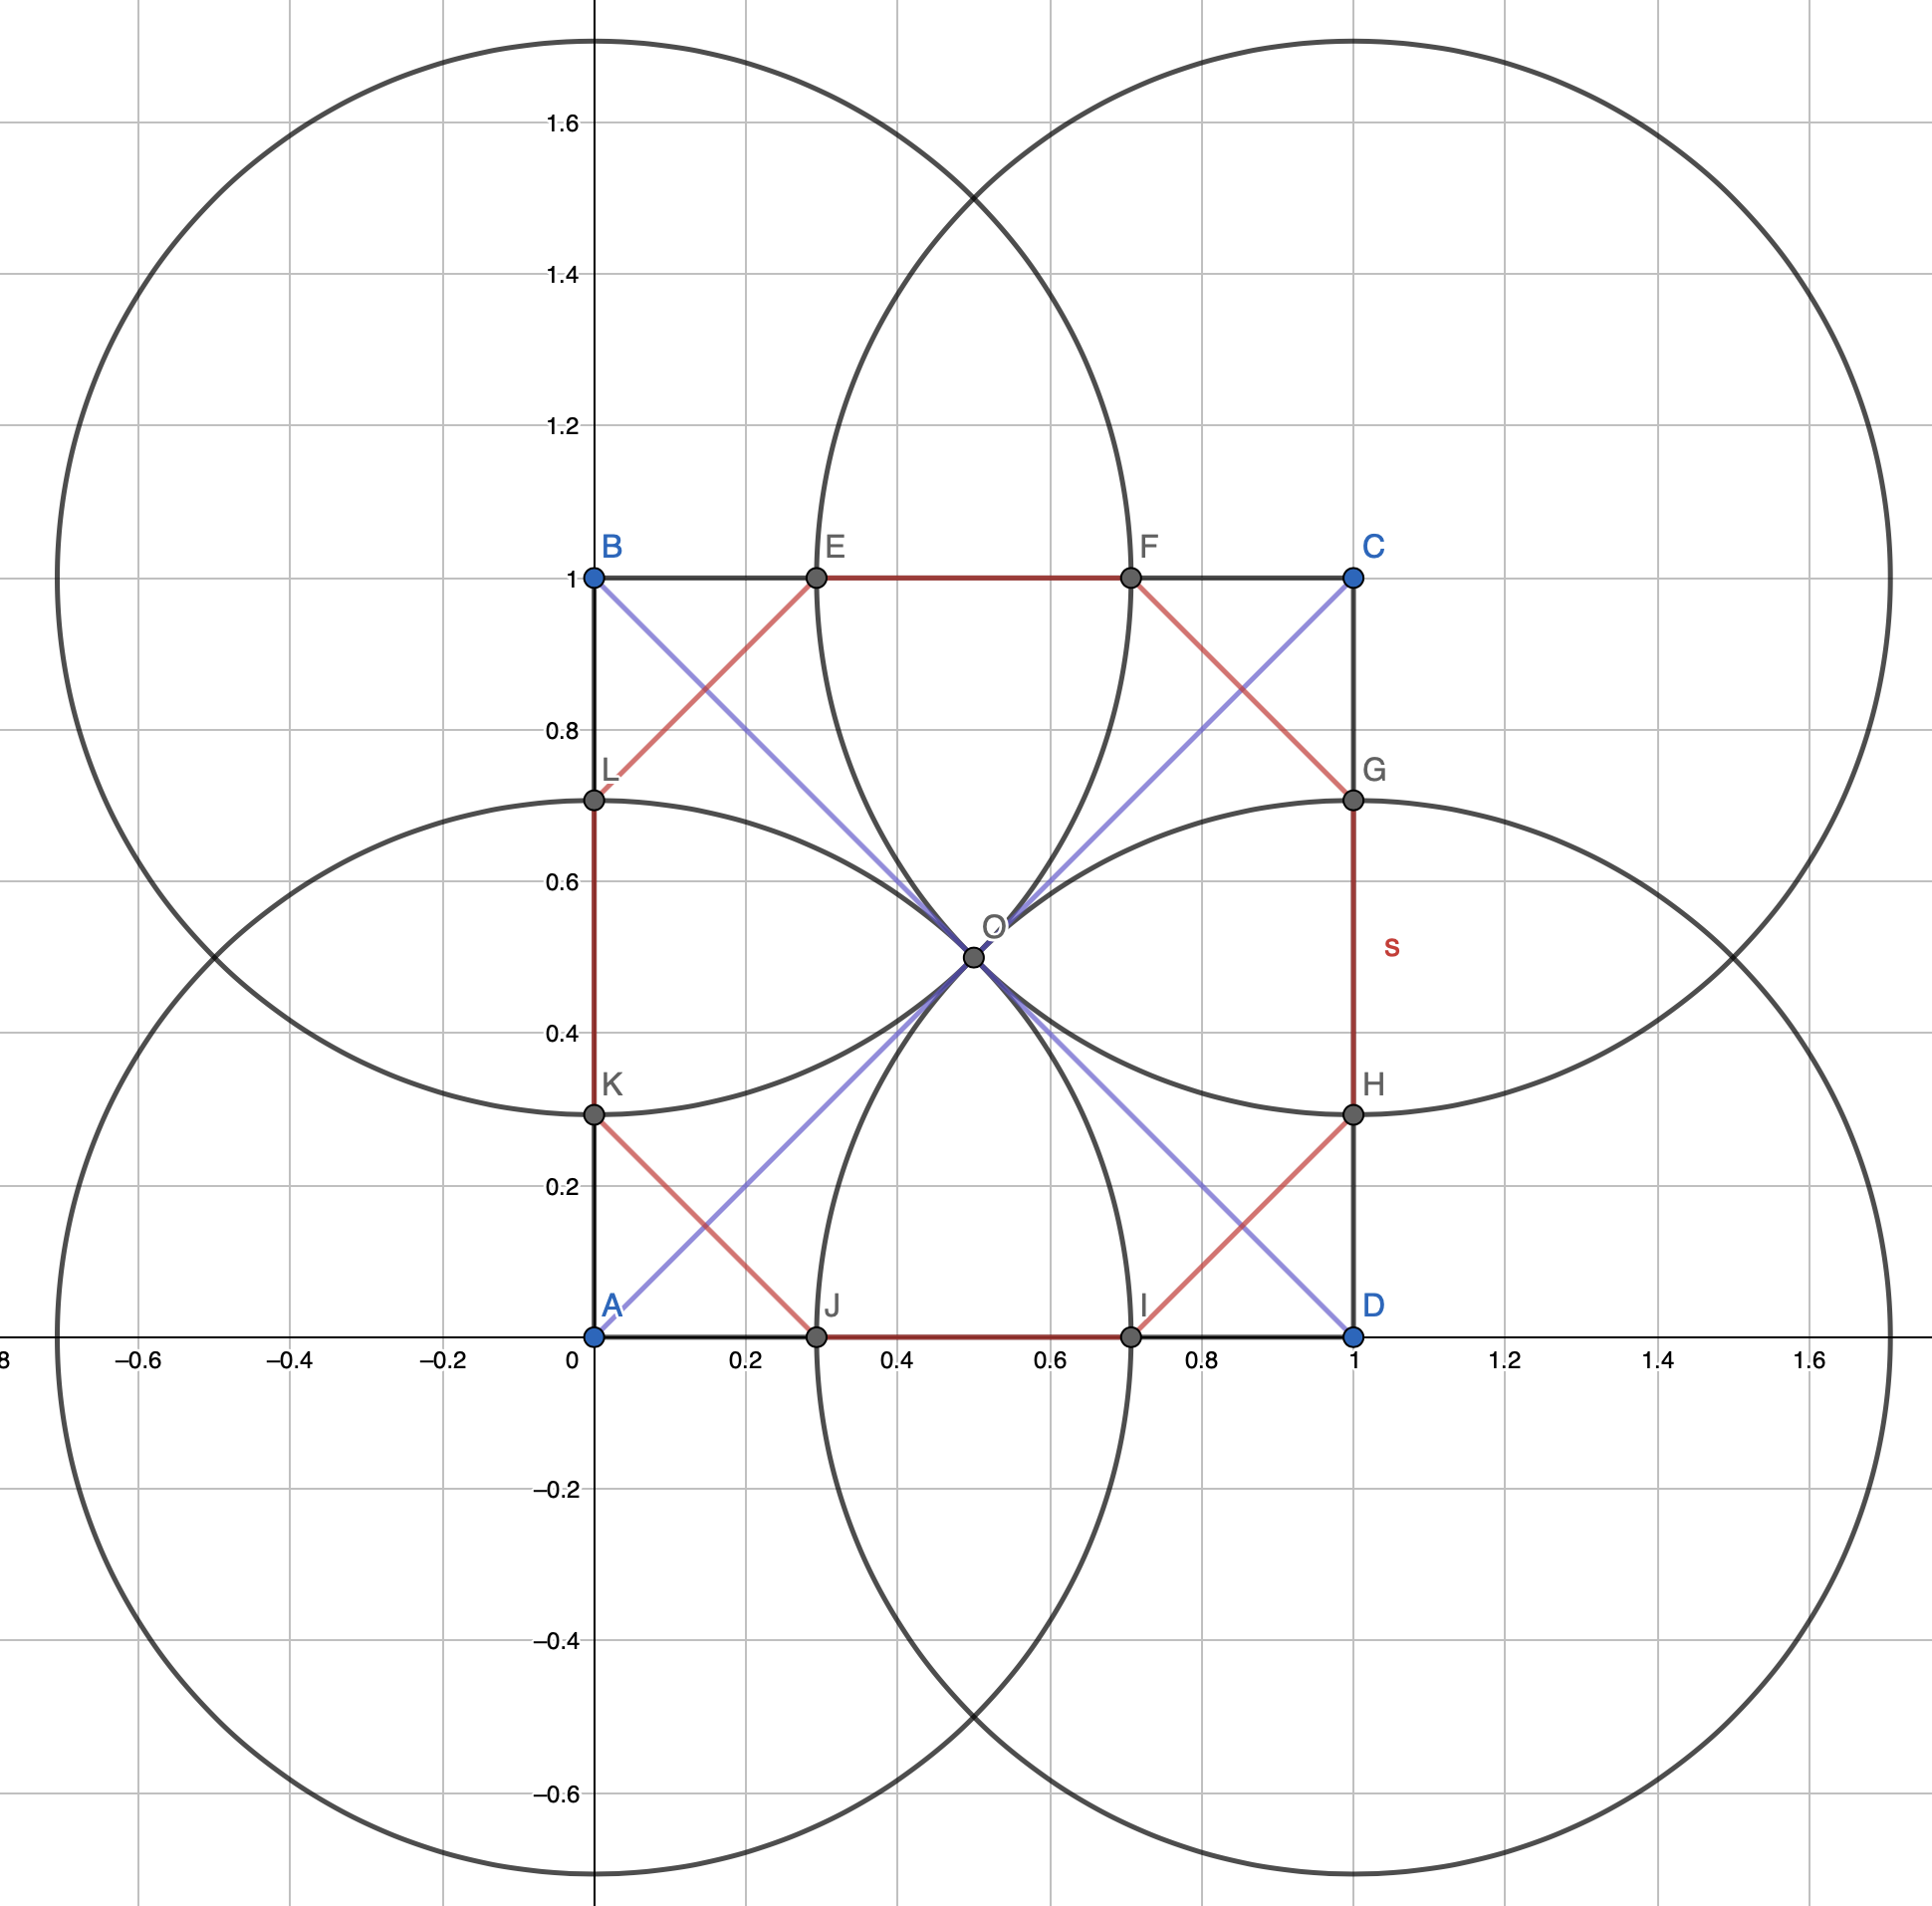
\includegraphics[scale=0.3]{fig/16b}
	%\caption{}
\end{figure}


\newpage

% ------------------------------
% 3.24
% ------------------------------
\begin{exer}[3.24]
Construct $\sqrt{5} $.
\end{exer}

\begin{figure}[H]
	\centering
	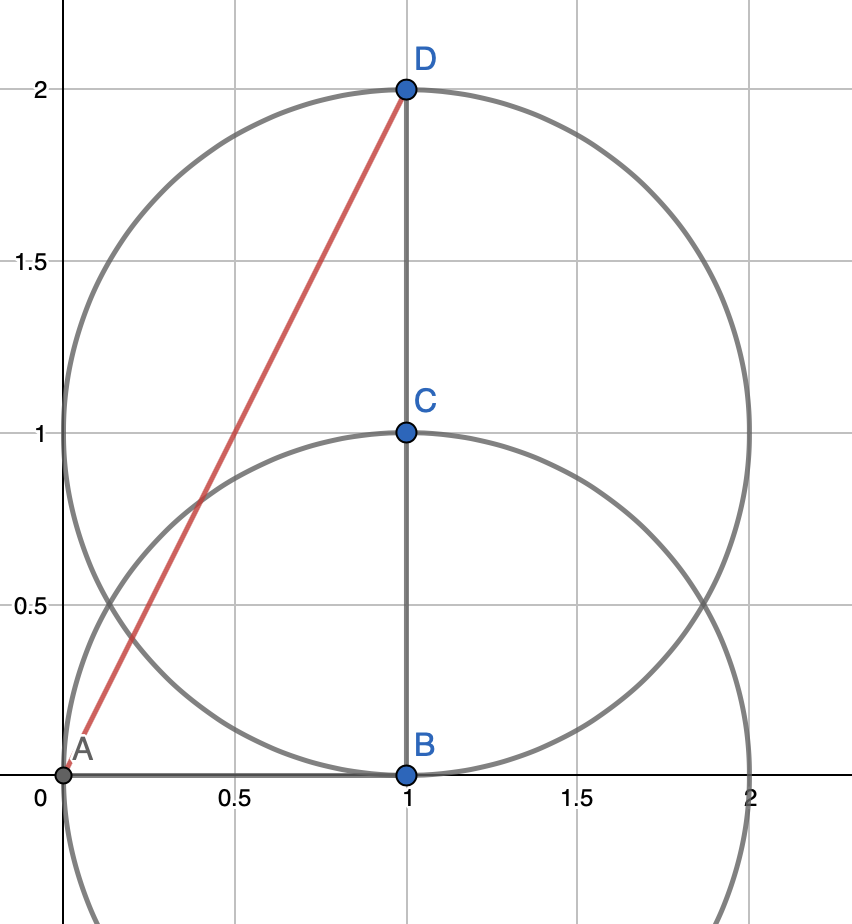
\includegraphics[scale=0.4]{fig/24}
	%\caption{}
\end{figure}

Take points $A$ and $B$ that are a distance 1 apart from each other. Construct the perpendicular to $AB$ through $B$, then choose a point at distance 2 from $B$ on it:
\begin{itemize}
	\item First choose an intersection point of the perpendicular bisector and $\mathcal{C}_{B}(|AB|)$, and label it $C$.
	\item The circle $\mathcal{C}_{C}(|BC|)$ intersects the perpendicular bisector at two points: $B$ and some other point. Label this other point $D$. Since $|AB|=|BC|=1$, the point $D$ is distance 2 from $B$.
\end{itemize}
By the Pythagorean Theorem, $|AC| = \sqrt{5} $.

\newpage

% ------------------------------
% 3.26
% ------------------------------
\begin{exer}[3.26]
Construct the geometric mean $\sqrt{ab} $.
\end{exer}

\begin{figure}[H]
	\centering
	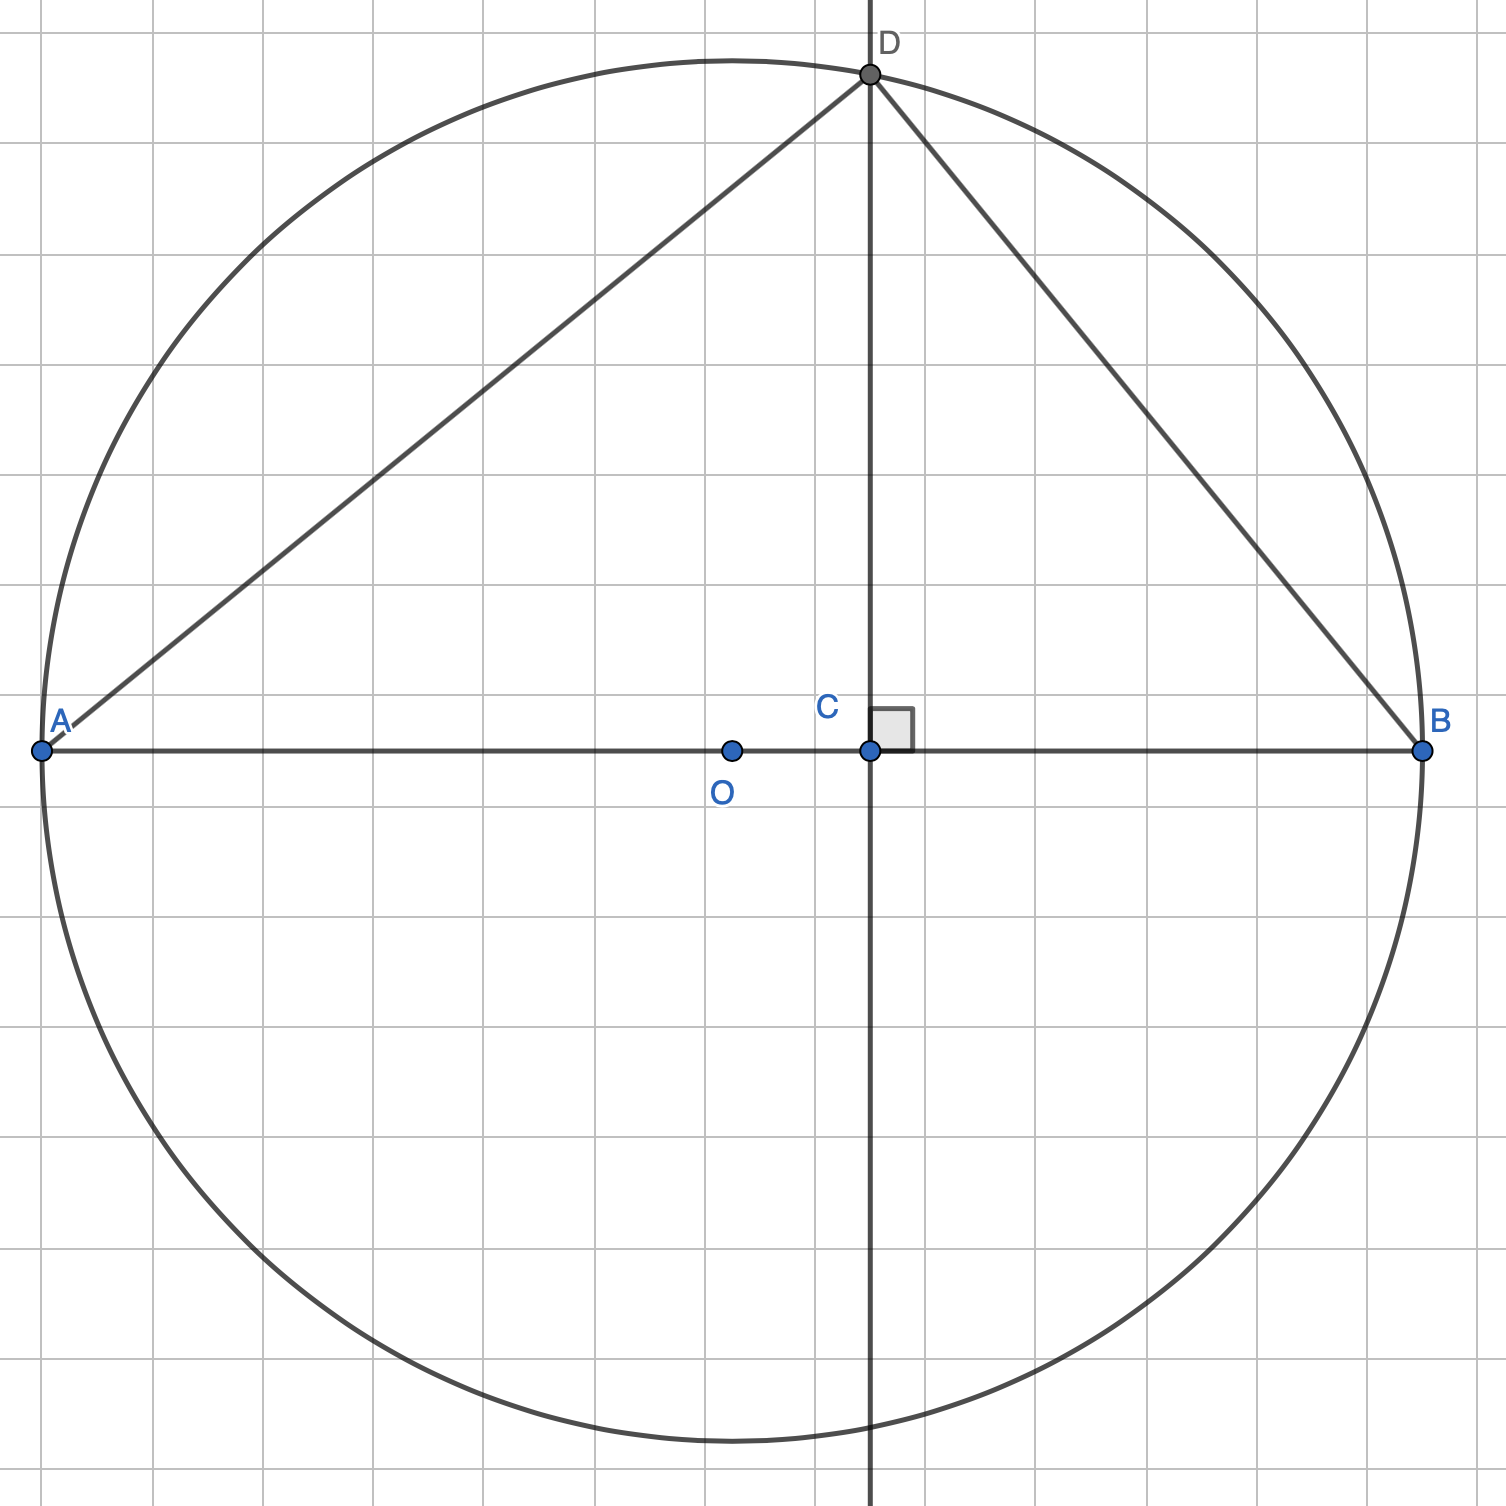
\includegraphics[scale=0.3]{fig/26}
	%\caption{}
\end{figure}

Take points $A$ and $C$ that are a distance $a$ away, then find a point $B$ on the extension of $AC$ that is a distance $b$ away from $C$. Now find the midpoint $O$ of $AB$, and use it to construct the circle $\mathcal{C}_{O}(|AO|)$.

Construct the perpendicular to $AB$ through $C$ and call one of its intersections with the circle $D$. By symmetry, the power of the point $C$ is $|CD|^2 = |AC| |BC| = a b$, so $|CD| = \sqrt{ab} $.

\newpage

% ------------------------------
% 3.33
% ------------------------------
\begin{exer}[3.33]
Construct a regular pentagon inscribed in a radius 4 circle.
\end{exer}

Suppose $|AB|=1$, then as in Exercise 3.24, we can construct a triangle with legs 1 and 2 and hypotnuse $\sqrt{5} $, as pictured below.

\begin{figure}[H]
	\centering
	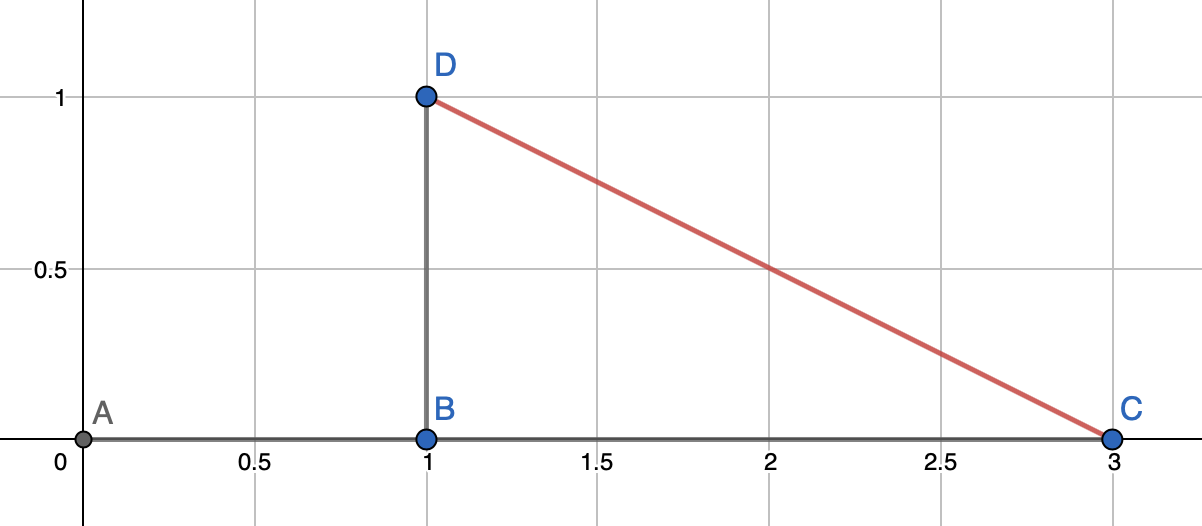
\includegraphics[scale=0.3]{fig/33a}
	%\caption{}
\end{figure}

Now construct the point $E$ by taking the intersection of $\mathcal{C}_{D}(|BD|)$ with $CD$. Note that $|CE|=\sqrt{5} -1$. Now take a perpendicular line of $FC$ through $E$, and mark its intersections with $\mathcal{C}_{C}(|CF|)$ as $G$ and $J$. Now mark the farther intersection points of $\mathcal{C}_J(|CJ|)$ and $\mathcal{C}_{G}(|CG|)$ with $\mathcal{C}_C(|CF|)$ as $H$ and $I$. Then $FGHIJ$ is our desired pentagon.

\begin{figure}[H]
	\centering
	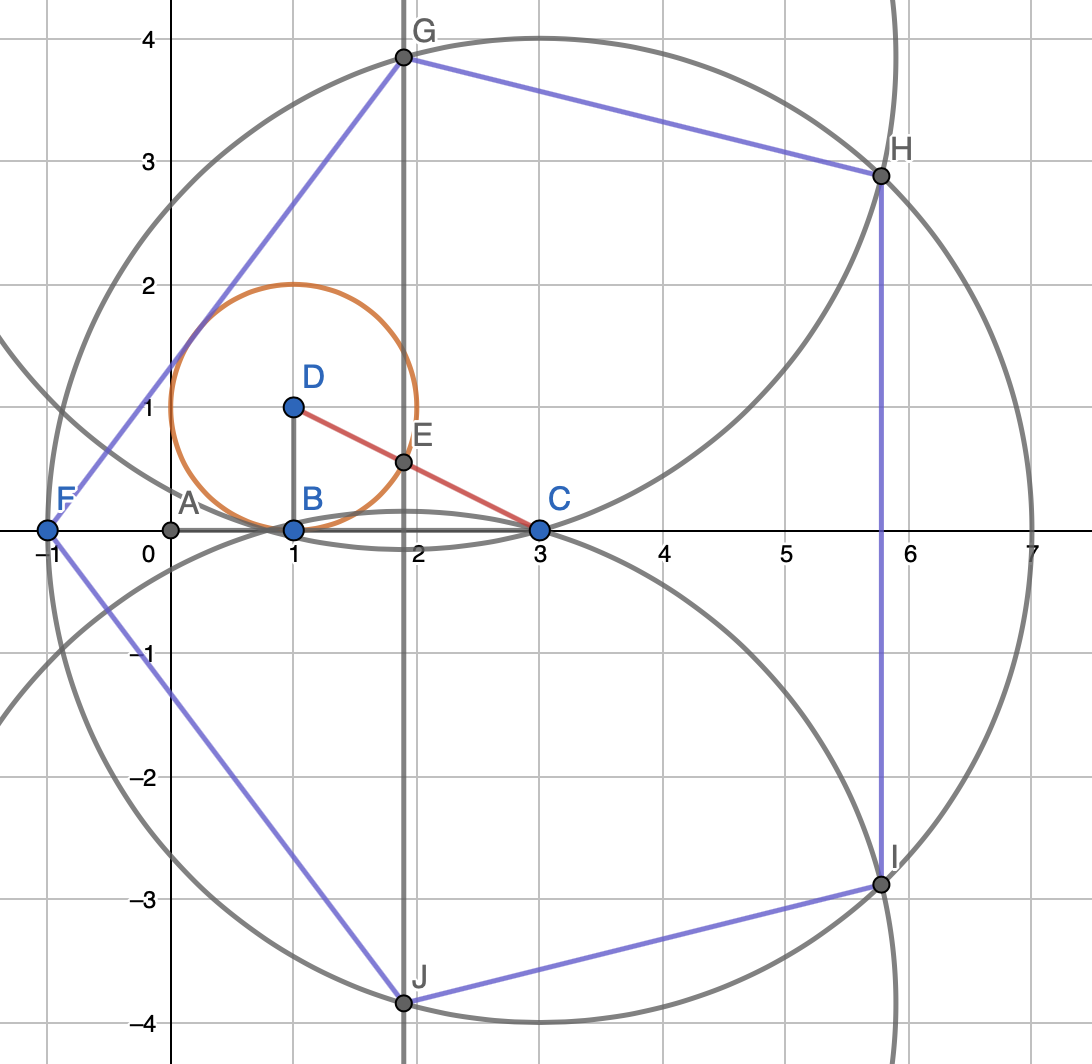
\includegraphics[scale=0.5]{fig/33b}
	%\caption{}
\end{figure}

\newpage

% ------------------------------
% 3.40
% ------------------------------
\begin{exer}[3.40]
Prove the angle sum formulas with Euler's formula.
\end{exer}

On one hand, we have
\begin{align*}
	e^{i(\alpha+\beta)} &= \cos(\alpha+\beta) + i \sin (\alpha+\beta).
\end{align*}
But this also evalutes to
\begin{align*}
	e^{i(\alpha+\beta)} &= e^{i\alpha}e^{i\beta} \\
			    &= \big( \cos\alpha+i\sin\alpha \big) \big( \cos\beta + i\sin\beta \big) \\
			    &= \cos \alpha\cos\beta - \sin\alpha\sin\beta + i\big( \sin \alpha\cos\beta+\cos\alpha\sin\beta \big).
\end{align*}
Equating these two then gives
\begin{align*}
	\sin(\alpha+\beta) &= \sin \alpha\cos\beta+\cos\alpha\sin\beta, \\
	\cos(\alpha+\beta) &= \cos \alpha\cos\beta - \sin\alpha\sin\beta,
\end{align*}
as desired.

\newpage

% ------------------------------
% 3.55
% ------------------------------
\begin{exer}[3.55]
	Is it possible to construct a triangle $\Delta ABC$ with $\angle BAC = 20\degree$, $|AB|=4$, and $|AC| = 2 \sqrt{3} $?
\end{exer}

No, it is not possible. Suppose $20\degree$ were constructible, then we could also construct $40\degree$. But $40\degree$ is the innermost angle of each triangle composing a 9-gon, so the 9-gon would also be constructible. But by Theorem 3.49, the 9-gon cannot be constructed. Thus we cannot construct our desired $\Delta ABC$.

\newpage

\end{document}
